\documentclass[%
 reprint,
 amsmath,amssymb,
 aps,
]{revtex4-1}

\usepackage{graphicx}
\usepackage{dcolumn}
\usepackage{bm}

\begin{document}

\preprint{APS/123-QED}

\title{D\'inamica molecular}

\author{Felipe Gonzalez}

\affiliation{%
 Departamento de F\'\i sica, Facultad de Ciencias Exactas y Naturales, Universidad de Buenos Aires,\\
 Pabell\'on I, Ciudad Universitaria, 1428 Buenos Aires, Argentina.
}

\date{\today}

\begin{abstract}

Se estudi\'o la evolucion de un sistema NVE bajo un potencial de Lennard Jones,
de caracter peri\'odico, integrado por el algoritmo de Velocity Verlet.

\end{abstract}

\maketitle

\section{Introducci\'on}

La d\'inamica molecular es una t\'ecnica de simulaci\'on que permite estudiar la
interacci\'on de \'atomos y mol\'eculas bajo la acci\'on de un potencial
particular, as\'i permitiendo la visualizacion del movimiento de las
part\'iculas. Esta t\'ecnica fue concebida dentro de la física te\'orica en fin
de entender la evoluci\'on de las magnitudes termodin\'amicas desde las
caracter\'isticas del sistema microsc\'opico, y ahora es ampliamente utilizada
en el campo de la biof\'isica y la ciencia de materiales.

El caso de estudio de este trabajo es un sistema NVE, en el cual se encuentran
fijas el numero de part\'iculas, el volumen y la energ\'ia total, cuya
interacci\'on esta caracterizada por un potencial de Lennard Jones.

\subsection{Potencial de Lennard Jones}

El potencial de Lennard Jones es el potencial can\'onico utilizado para simular
la interacci\'on entre moleculas, y su forma funcional es la siguiente:

\begin{equation}
  V(r) = 4 \epsilon \left[
    \left(
      \frac{\sigma}{r ^ 12}\right) - \frac{\sigma}{r ^ 6}
    \right)
  \right]
\end{equation}

Vemos que el potencial tiene 2 distintas componentes, una repulsiva que va
como $\propto \frac{1}{r ^ 12}$ y otra atractiva que va como
$\propto \frac{1}{r ^ 6}$. La primera de ellas viene a modelar la repulsi\'on de
Pauli entre los orbitales electr\'onicos, siendo de menor alcance, y la segunda
modela la atracci\'on electromagn\'etica, cuyo decaimiento de es cuadr\'atico
sino mayor siendo que los momentos monopolares de las p\'articulas son nulos.
La forma funcional de este potencial es la que se muestra en la figura
\ref{lj_potential}.

\begin{figure}
  \begin{center}
  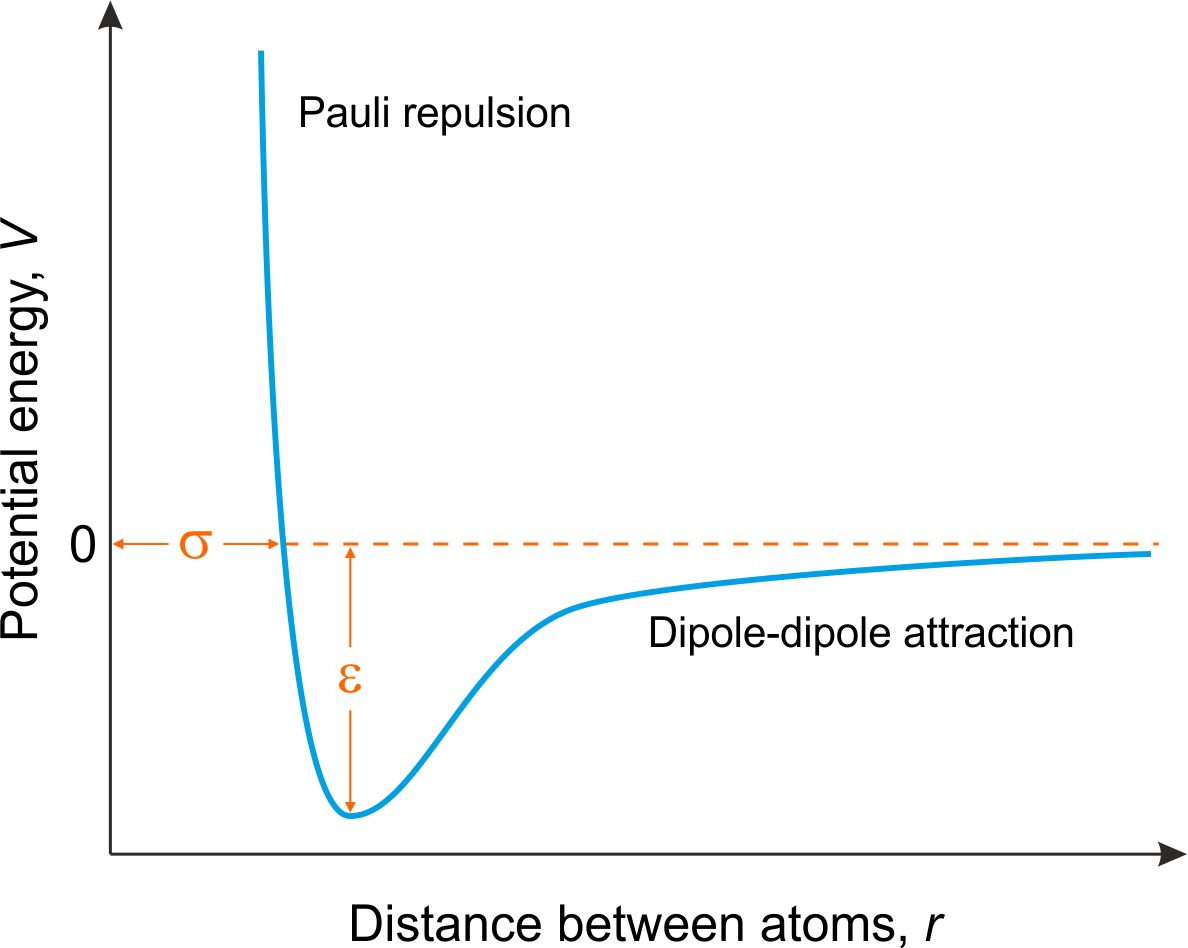
\includegraphics[scale=0.62]{/images/lj_potential.png}
  \caption{Forma funcional del potencial de Lennard Jones.}
  \label{lj_potential}
\end{center}
\end{figure}

Para integrar este potencial es necesario un integrador simpl\'ectico ya que
estamos bajo la presencia de un sistema f\'isico cuya energ\'ia se conserva.
Por esta razon se utiliza el algoritmo Velocity Verlet.

\subsection{Velocity Verlet}

El algoritmo de Velocity Verlet es un integrador simpl\'ectico de muy bajo
costo computacional cuando la aceleraci\'on de las particulas no depende de la
velocidad de las mismas. Haciendo uso de esta propiedad se deriva un integrador
que tiene los beneficios de un integrador implicito (conservaci\'on del volumen
en el espacio de fases) y de un integrador explicito (bajo costo computacional).

El algoritmo consiste en evolucionar la posicion y velocidad de las particulas
de la siguiente manera:

\begin{equation}
  \left \{
  \begin{matrix}
    x(t + h) = x(t) + h\.v(t) + \frac{h ^ 2}{2} f(t) //
    v(t + h) = v(t) + h \frac{f(t) + f(t + h)}{2},
  \end{matrix}
  \right .
\end{equation}

siendo $x$, $v$ y $f$ la posicion, velocidad y fuerza del cuerpo en cuesti\'on
y $h$ el paso temporal. Vemos que la dependencia de $v(t + h)$ con $f(t + h)$
indicar\'ia que nos encontramos frente a una ecuaci\'on implicita, sin embargo
esto no es asi ya que $f$ no depende de $v$, sino solo de $x$.

Sabemos adem\'as que para poder simular el sistema es necesario darle una
condici\'on inicial, sin embargo no tenemos ninguna garant\'ia de que la
condici\'on inicial fijada sea un estado representativo de los para\'ametros
termodinamicos provistos, siendo que a priori uno no sabe si se encuentra en
equilibrio. Esto indica que es necesario un periodo de termalizaci\'on para que
el sistema llegue al equilibrio.

\subsection{Termalizaci\'on}

Cualquier sistema siendo simulado debe comenzar por una condicion inicial
impuesta la cual puede o no ser representativa del mismo. Asi, se debe tener
especial cuidado en dejar la suficiente cantidad de pasos para asegurar que el
sistema se encuentra en equilibrio antes de realizar mediciones sobre el mismo.

En el caso de din\'amica molecular existen diversos metodos para entender si
el sistema esta termalizado. Uno de ellos es el coeficiente de Verlet, que da
una medida del desorden de las particulas entendiendo desorden como el
apartamiento de un arreglo simple c\'ubico, siendo este el arreglo inicial.
Este coeficiente se calcula de la siguiente manera.

\begin{equation}
  \left \{
    \begin{matrix}
      \lambda_x = \frac{1}{N} \sum_{i = 1}^N \cos \left( \frac{2 \pi m}{L} x_i - \pi \right) \\
      \lambda_y = \frac{1}{N} \sum_{i = 1}^N \cos \left( \frac{2 \pi m}{L} y_i - \pi \right) \\
      \lambda_z = \frac{1}{N} \sum_{i = 1}^N \cos \left( \frac{2 \pi m}{L} z_i - \pi \right)
    \end{matrix}
    \lambda = \frac{1}{3} (\lambda_x + \lambda_y + \lambda_z) ,
  \right .
\end{equation}

siendo $\lambda$ el coeficiente, $L$ el lado de la caja cubica y $m$ la
cantidad de particulas por lado. Tenemos que el coeficiente comienza siendo
id\'enticamente $1$, y se va reduciendo a medida que las particulas se mueven
de este arreglo.


\section{Resultados}

Durante el transcurso del trabajo se utilizaron unidades reducidas.

\subsection{Termalizaci\'on}

Se comenzo por estudiar la termalizaci\'on del sistema, en pos de evitar tomar
mediciones fuera del equilibrio. Para esto, se utilizaron diversos criterios
para evitar tomar una decision sesgada. Se comenzo por estudiar la evoluci\'on
de la energ\'ia en funcion del tiempo.

\begin{figure}
  \begin{center}
  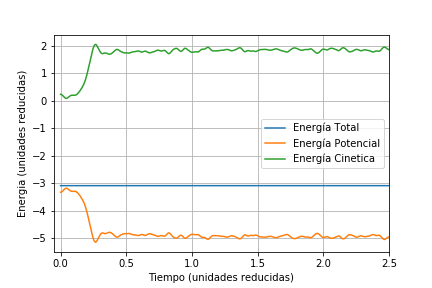
\includegraphics[scale=0.62]{/images/e_vs_t.png}
  \caption{Energia total, potencial y cin\'etica en funci\'on del tiempo para
  un sistema de 512 part\'iculas, cuyos parametros iniciales son
  $\rho = 0.8422$ y $T = 0.728$.}
  \label{e_vs_t}
\end{center}
\end{figure}

Vemos que la energ\'ia total se mantiene estable, lo que era esperable de un
integrador simpl\'ectico, sin embargo existe una transferencia neta de
energ\'ia potencial a cin\'etica entre $t \in [0, 0.5]$. Vemos que una vez pasado
este tiempo siguen existiendo transferencias, pero son simples fluctuaciones
debido a que se tiene una cantidad finita de particulas. De esta manera, se
podr\'ia entender que una vez pasado $t = 2.5$ se llega a un estado de
equilibrio, representativo del sistema a analizar, cuya temperatura no es igual
a la que fue seteada al principio de la simulaci\'on.

Otro par\'ametro a seguir para entender la termalizaci\'on del sistema es el
coeficiente de Verlet.

La evoluci\'on del coeficiente de Verlet en funci\'on del tiempo para el
sistema propuesto se encuentra en la figura \ref{verlet_vs_t}}.

\begin{figure}
  \begin{center}
  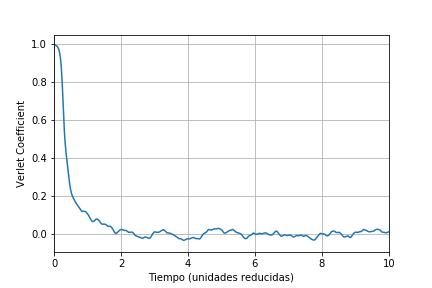
\includegraphics[scale=0.62]{/images/verlet_vs_t.png}
  \caption{Coeficiente de Verlet en funcion del tiempo para un sistema de 512
  part\'iculas, cuyos parametros iniciales son $\rho = 0.8422$ y $T = 0.728$.}
  \label{verlet_vs_t}
\end{center}
\end{figure}

Vemos que se puede ver que para $t \simeq 0.5$ el sistema sigue con un
coeficiente de Verlet considerable lo que nos deja entender que por mas que se
realiz\'o la transferencia de energ\'ia potencial a energia cin\'etica, sigue
existiendo una noci\'on de orden en el sistema, remanente del estado inicial.
Esto indica que para poder realizar mediciones confiables el sistema debe
dejarse termalizar al menos hasta llegar a $t = 2$.

\subsection{Transiciones de Fase}

Una vez entendida la termalizaci\'on del sistema, se analizan las transiciones
de fase que atraviesa el sistema. Para ello, se realiza un barrido de
$\rho \in [0.4, 0.8]$ con paso de $0.01$ y $T \in [0.4, 2]$ con paso de $0.1$,
para un sistema de $125$ part\'culas. Tenemos que en este rango de parametros,
para distintas combinaciones de los mismos, esperamos que el sistema transicione
de estado gaseoso a l\'iquido.

La literatura nos dice que deberiamos esperar un gas para $\rho = 0.4$ y $T = 2$,
mientras que para $\rho = 0.4$ y $T = 0.4$ deberiamos tener un l\'iquido. Para
chequear esta hipotesis, calcula la funci\'on de distribucion radial $g(r)$
sobre estos puntos, para ver si el comportamiento de estas funciones son las
esperadas para su estado.

Sobre la figura \label{liquido} tenemos la funci\'on $g(r)$ para $\rho = 0.4$ y
$T = 0.4$, condici\'on sobre la cual esperamos tener un l\'iquido. Vemos que
la funci\'on tiene oscilaciones sobre esta funci\'on que son las
caracter\'isticas de un l\'iquido, en la cual se puede ver un poco de
oscilaciones pero mueren r\'apido. Por el otro lado, en la figura \label{gas}
tenemos $g(r)$ para $\rho = 0.4$ y $T = 2$. En este caso se cumple que la caida
despues del pico inicial es constante y no existen oscilaciones, lo cual es
compatible con un gas. Por completitud tenemos en la figura \label{solido} la
funci\'on $g(r)$ para $\rho = 1.5$ y $T = 0.4$, en donde la literatura predice
la fase s\'olida. Vemos que en este caso se tiene muchas mas oscilaciones,
tipicas del estado s\'olido.

\begin{figure}
  \begin{center}
  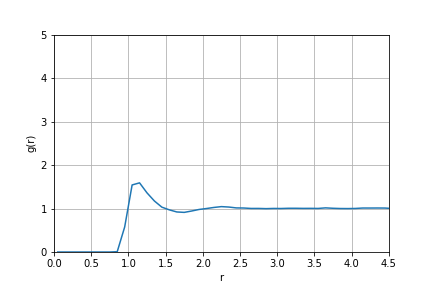
\includegraphics[scale=0.62]{/images/gas.png}
  \caption{$g(r)$ para $\rho = 0.4$ y $T = 2$. Vemos que la forma funcional
  es la esperada para un gas.}
  \label{gas}
\end{center}
\end{figure}

\begin{figure}
  \begin{center}
  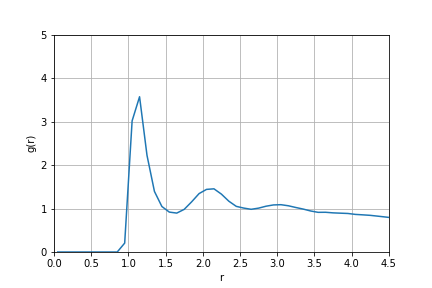
\includegraphics[scale=0.62]{/images/liquido.png}
  \caption{$g(r)$ para $\rho = 0.4$ y $T = 0.4$. Vemos que la forma funcional
  es la esperada para un gas.}
  \label{liquido}
\end{center}
\end{figure}

\begin{figure}
  \begin{center}
  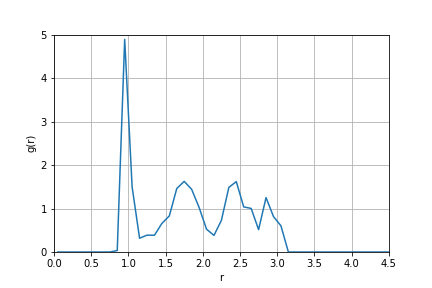
\includegraphics[scale=0.62]{/images/solido.png}
  \caption{$g(r)$ para $\rho = 1.5$ y $T = 0.4$. Vemos que la forma funcional
  es la esperada para un gas.}
  \label{solido}
\end{center}
\end{figure}

De este manera sabemos que entre estos valores debe existir la transici\'on. En
la figura \label{e_vs_t_rho_0.4} tenemos la energia en funci\'on de la
temperatura para $\rho = 0.4$. Vemos que para las temperaturas mas bajas es
sistema tiene un comportamiento cualitativamente distinto que para las mas
altas, en particular se puede decir que para $T \simeq 1.2$ el comportamiento
se vuelve lineal para las temperaturas mayores, lo cual es razonable para un
gas debido a que imita el comportamiento de un gas ideal en donde no hay
interacci\'on, ya que la temperatura comienza a superar el potenciales. No solo
eso, sino que al realizar un ajuste lineal sobre este subconjunto de mediciones
tenemos que la pendiente es de $(1.76 \pm 0.04)$, la cual es compatible con el
valor te\'orico del calor espec\'ifico de $\frac{3}{2}$.

\begin{figure}
  \begin{center}
  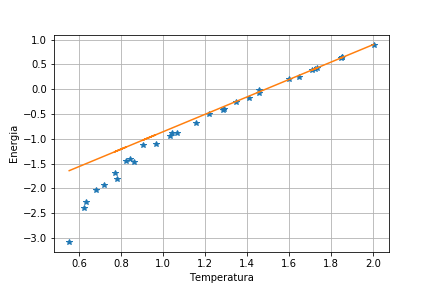
\includegraphics[scale=0.62]{/images/e_vs_t_rho_0.4.png}
  \caption{Energia en funci\'on de la temperatura para $\rho = 0.4$, vemos que
  se pueden apreciar 2 regimenes distintos a simple vista, siendo el segundo de
  caracter lineal. Se ajusto una recta para los datos cuya temperatura es
  mayor $1.5$, dando como resultado una pendiente de $(1.76 \pm 0.04)$.}
  \label{e_vs_t_rho_0.4}
\end{center}
\end{figure}

Algo interesante ocurre tambi\'en con la presi\'on. Tenemos que para el rango
estudiado, 

\section{Conclusiones}

\appendix
\bibliography{apspaper}  % Produces the bibliography via BibTeX.

\end{document}
